
\documentclass[letterpaper, 10 pt, conference]{ieeeconf}  % Comment this line out if you need a4paper

%\documentclass[a4paper, 10pt, conference]{ieeeconf}      % Use this line for a4 paper

\IEEEoverridecommandlockouts                           

\overrideIEEEmargins                                      % Needed to meet printer requirements.

%In case you encounter the following error:
%Error 1010 The PDF file may be corrupt (unable to open PDF file) OR
%Error 1000 An error occurred while parsing a contents stream. Unable to analyze the PDF file.
%This is a known problem with pdfLaTeX conversion filter. The file cannot be opened with acrobat reader
%Please use one of the alternatives below to circumvent this error by uncommenting one or the other
%\pdfobjcompresslevel=0
%\pdfminorversion=4

% See the \addtolength command later in the file to balance the column lengths
% on the last page of the document

% The following packages can be found on http:\\www.ctan.org
\usepackage{graphics} % for pdf, bitmapped graphics files
\usepackage{epsfig} % for postscript graphics files
\usepackage{mathptmx} % assumes new font selection scheme installed
\usepackage{times} % assumes new font selection scheme installed
\usepackage{tabularx}
\usepackage{graphicx}
\usepackage{amsmath}
\usepackage{amsfonts}
\usepackage{amssymb}
\usepackage{url}
\usepackage{cite}

\PassOptionsToPackage{hyphens}{url}
\usepackage{hyperref}


\title{\LARGE \bf
Tracking Hidden Caregiver Strain with Interview and Wearable Data
}


\author{%
Junen Xiao$^{1*}$%
\thanks{$^{1}$Junen Xiao is with the Department of Electrical and Computer Engineering, Rice University, Houston, TX 77005, USA (\texttt{jx57@rice.edu}).}%
}

\begin{document}

\maketitle
\thispagestyle{empty}
\pagestyle{empty}


%%%%%%%%%%%%%%%%%%%%%%%%%%%%%%%%%%%%%%%%%%%%%%%%%%%%%%%%%%%%%%%%%%%%
\begin{abstract}
Alzheimer’s disease spousal caregivers frequently experience high caregiver burden and loneliness, leading to sustained psychological stress. Given the association between chronic caregiving stress and adverse health outcomes, early identification of psychological risk in caregivers is essential for prevention.
Current approaches for stress inference typically rely on data from wearable sensors, together with standardized psychological scales. To capture the multidimensional nature of mental health, state-of-the-art approaches adopt multimodal modeling to improve predictive performance.
This study integrates wearable-derived data and interview-based text to classify caregivers into different psychological risk levels using the Perceived Stress Scale, Zarit Burden Interview, and UCLA Loneliness Scale. The classification performance of traditional machine learning models and large language models (Gemini 2.0, Llama 4, and GPT4o) is compared across different modality settings and prompting strategies.
\end{abstract}


%%%%%%%%%%%%%%%%%%%%%%%%%%%%%%%%%%%%%%%%%%%%%%%%%%%%%%%%%%%%%%%%%%%%%%%%%%%%%%%%
\section{INTRODUCTION}
Caring for a spouse with Alzheimer’s Disease (AD) constitutes a major source of emotional strain\cite{stress}. This chronic caregiving stress is linked to physiological stress responses, including increased pro-inflammatory activity and systemic inflammation, which can lead to adverse health outcomes. Timely detection of rising psychological strain is therefore essential. However, caregivers vary substantially in their resilience and vulnerability to stress. This emphasizes the need for personalized, timely stress detection to identify individuals at elevated risk and enable targeted support.

Validated self-report instruments such as the Perceived Stress Scale (PSS), Zarit Burden Interview (ZBI), and UCLA Loneliness Scale (UCLALS) are commonly used to assess caregiver psychological risk\cite{pss,ucla,ZBI} in caregiving studies, while passive sensing data from wearable devices capture continuous behavioral and physiological signals linked to stress-related processes\cite{smets2018large}. However, wearable-derived data alone may not adequately capture the subjective psychological experiences central to caregiving. This motivates a multimodal approach that uses interview-based text and wearable signals to estimate standard self-report psychological scales.

Nevertheless, robustly predicting self-report psychological scores from real-world data is challenging. Given the limited sample sizes, complex end-to-end deep learning models often struggle to generalize effectivel\cite{small_dataset}. Simpler machine learning models built on lightweight text representations (e.g., TF-IDF\cite{tf-idf} or Word2Vec\cite{word2vec}), often provide more stable results. At the same time, large language models (LLMs) provide a practical way to incorporate free-text interview data and text-formatted wearable-derived features, as they can be directly used for text encoding and scoring without requiring large task-specific datasets\cite{bert,llm_scoring}.

Based on the above motivations, our contributions can be summarized as follows:
\begin{itemize}
    
    \item We apply traditional text processing and machine learning models to classify high-risk groups for psychological scales (PSS, ZBI, and UCLALS) using both interview text and wearable-derived features.
    
    \item We design caregiver-centered and psychologist-centered prompting strategies to enable Gemini 2.0, Llama4, and GPT4o to perform the same classification task.

    \item We conduct ablation studies with wearable-only and interview-only settings to evaluate the contribution of each data modality.
\end{itemize}

\section{Method}
\begin{figure*}[!t]
    \centering
    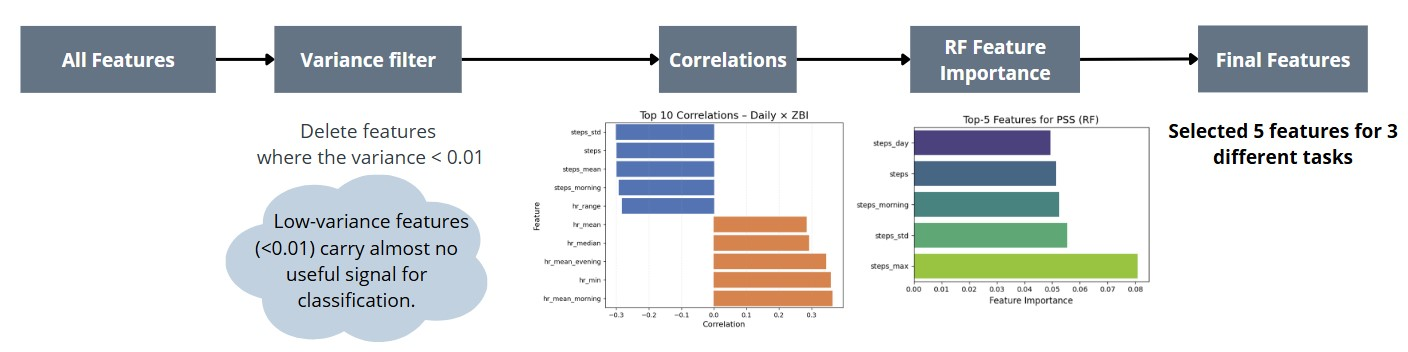
\includegraphics[width=\linewidth]{Feature workflow.jpg}
    \caption{Overview of the feature selection workflow.}
    \label{fig:feature_workflow}
\end{figure*}
\subsection{Dataset}
This study enrolled 32 caregivers (28 female and 4 male) of patients with Alzheimer’s disease. Participants were between 50 and 89 years of age (mean age = 71, SD = 7.04). Most participants identified as White (27), followed by African American (4), and Other (1).

Participants wore Fitbit devices during a 7-day study block, which continuously recorded minute-level heart rate, sleep status, and step count data. In addition, participants completed an interview consisting of 28 questions. These questions covered categories such as caregiving background, caregiving experiences and stress levels. At the end of the study, participants completed the standardized surveys (PSS\cite{pss}, UCLALS\cite{ucla}, and ZBI\cite{ZBI}), which served as ground-truth labels in this study.

We categorized participants into two groups using established cut-off criteria for the 3 scales respectively. The binary classification criteria and label distribution for the psychological scales are summarized in Table~\ref{tab:label_distribution}.

\begin{table}[t]
\centering
\caption{Binary classification rules and label distribution for psychological scales.}
\label{tab:label_distribution}
\begin{tabular}{lccc}
\hline
\textbf{Scale} & \textbf{Binary Rule} & \textbf{Low Risk (n,\%)} & \textbf{High Risk (n,\%)} \\
\hline
PSS\cite{pss} & $\geq 14 \rightarrow 1$ & 10 (31.25\%) & 22 (68.75\%) \\
UCLALS\cite{ucla} & $\geq 35 \rightarrow 1$ & 8 (25.00\%) & 24 (75.00\%) \\
ZBI\cite{ZBI} & $\geq 21 \rightarrow 1$ & 12 (37.50\%) & 20 (62.50\%) \\
\hline
\end{tabular}
\end{table}

\subsection{Wearable Feature Extraction and Selection}
We extracted sleep, daily, and rhythm features from the Fitbit data of each participant. Sleep features mainly consist of the duration in different stages of sleep, including asleep, restless, and awake states. The Sleep Regularity Index (SRI)~\cite{sri} was also calculated based on the whole-day sleep states at minute-level resolution. The higher SRI indicates greater regularity in sleep patterns.

Daily features were derived from minute-level heart rate and step data. Heart rate features included summary statistics and the proportion of minutes with elevated heart rate (HR$>$100 bpm). Activity features included step statistics, active and sedentary time proportions, and step entropy. Features were computed separately for different times of day (morning, afternoon, evening, and night).

Rhythm features were extracted from hourly aggregated heart rate and step data\cite{heartrate}. To ensure reliable estimation, participants with at least five complete days of 24-hour data were included. Rhythm features were then derived using both nonparametric metrics and parametric cosinor analysis. Additional statistics describing deviations from the participant-specific 24-hour activity template were computed to capture rhythm stability and variability. 

A multi-stage feature selection pipeline (Fig.~\ref{fig:feature_workflow}) was then used, which includes variance filtering, correlation analysis, and Random Forest feature importance. As a result, the top five features were selected for each classification task.

\subsection{Machine Learning Models}
Machine learning models were trained to classify participants into different risk groups based on their wearable features and interview text. Lightweight text representations, including TF-IDF\cite{tf-idf} and Word2Vec\cite{word2vec}, were adopted to encode the interview-based text. After obtaining the text representations, an early fusion strategy was applied to integrate wearable data and text features by concatenating them into a single feature vector.

We utilized models such as Support Vector Machine (SVM)\cite{cortes1995support}, XGBoost (XGB)\cite{xgboost}, Random Forest (RF)\cite{rf}, and K-Nearest Neighbors (KNN)\cite{knn} for binary classification. Two simple baselines, namely the majority-class baseline and the probabilistic random baseline, were also adopted for performance comparison.  Due to the limited sample size, Leave-One-Out Cross-Validation (LOOCV)\cite{loocv} was employed, in which one participant was held out as the test sample while the remaining participants were used for training. Model performance was evaluated using accuracy, precision, recall, and F1 score.

\subsection{Prompt Engineering Strategies}
An LLM-based approach was also adopted for identification of different risk levels among participants. In this framework, interview transcripts and wearable features were integrated at the prompt level. Specifically, the interview text was provided directly as natural language input, while wearable features were converted into textual descriptions with feature names, explanations, and numeric values. These multimodal inputs were then combined within a single prompt to guide the model to classify the participants.

Given that LLM predictions can be sensitive to task framing and instructed perspective \cite{rethinking, patient}, we designed six prompt strategies: Caregiver--Score Prediction (C\_S), Caregiver--Direct Classification (C\_C), Expert--Informed--Score Prediction (EI\_S), Expert--Informed--Direct Classification (EI\_C), Expert--Uninformed--Score Prediction (EU\_S), and Expert--Uninformed--Direct Classification (EU\_C). These strategies vary along three dimensions: perspective (caregiver vs. expert), task framing (classification vs. score prediction), and questionnaire information (uninformed vs. informed). For score prediction, the predicted scores were converted to binary labels using a predefined cut-off. We then conducted zero-shot inference with three models: Gemini~2.0, GPT-4o, and Llama~4.



\begin{figure}[t]
    \centering
    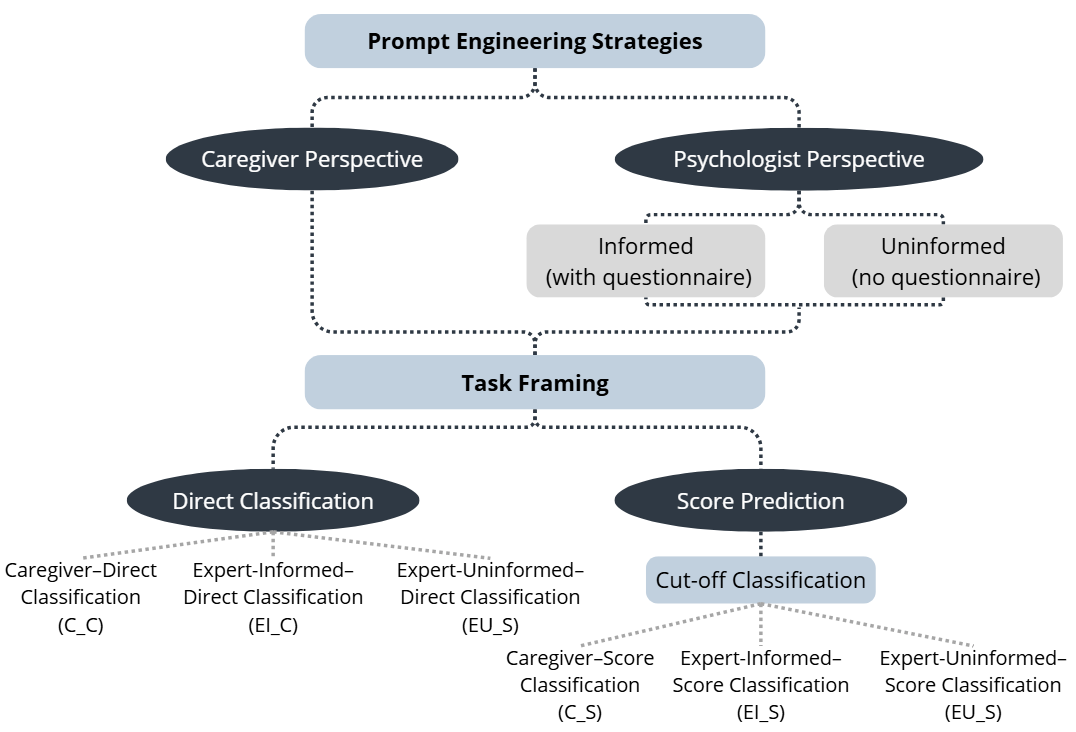
\includegraphics[width=\linewidth]{Prompt_Engineering.png}
    \caption{Overview of the prompt engineering strategies.}
    \label{fig:prompt_engineering}
\end{figure}

\section{Results}
For each psychological risk classification task, we compare the best-performing ML model, the best prompt strategy for each LLM (Gemini~2.0, GPT-4o, and Llama 4) and the two baselines. Tables\ref{tab:method_results_1}, \ref{tab:method_results_2}, and \ref{tab:method_results_3} present the results for PSS, ZBI, and UCLALS, respectively.

\begin{table}[h]
\centering
\caption{Performance comparison of different methods for PSS.}
\label{tab:method_results_1}
\resizebox{\columnwidth}{!}{
\begin{tabular}{lcccc}
\hline
Method & Accuracy & Recall & F1 & Precision \\
\hline
Majority Vote & 0.69 & 1.00 & 0.82 & 0.69 \\
Random Vote & 0.55 $\pm$ 0.08 & 0.67 $\pm$ 0.10 & 0.67 $\pm$ 0.07 & 0.68 $\pm$ 0.06 \\
W2V+SVM & 0.78 & 0.86 & 0.84 & 0.83 \\
Gemini\_EI\_C & 0.71 $\pm$ 0.03 & 0.95 $\pm$ 0.03 & 0.82 $\pm$ 0.02 & 0.72 $\pm$ 0.02 \\
Llama4\_EI\_C & 0.64 $\pm$ 0.03 & 0.93 $\pm$ 0.04 & 0.78 $\pm$ 0.02 & 0.67 $\pm$ 0.01 \\
GPT4o\_EU\_S & 0.73 $\pm$ 0.03 & 0.95 $\pm$ 0.02 & 0.83 $\pm$ 0.02 & 0.74 $\pm$ 0.02 \\
\hline
\end{tabular}
}
\end{table}

\begin{table}[t]
\centering
\caption{Performance comparison of different methods for ZBI. }
\label{tab:method_results_2}
\resizebox{\columnwidth}{!}{
\begin{tabular}{lcccc}
\hline
Method & Accuracy & Recall & F1 & Precision \\
\hline
Majority Vote & 0.63 & 1.00 & 0.77 & 0.63 \\
Random Vote & 0.52 $\pm$ 0.08 & 0.61 $\pm$ 0.11 & 0.61 $\pm$ 0.08 & 0.61 $\pm$ 0.07 \\
TF-IDF+SVM & 0.56 & 0.65 & 0.65 & 0.65 \\
Gemini\_C\_C & 0.81 $\pm$ 0.02 & 1.00 $\pm$ 0.00 & 0.87 $\pm$ 0.01 & 0.76 $\pm$ 0.02 \\
Llama4\_C\_C & 0.77 $\pm$ 0.03 & 1.00 $\pm$ 0.00 & 0.84 $\pm$ 0.02 & 0.73 $\pm$ 0.03 \\
GPT4o\_EI\_S & 0.80 $\pm$ 0.02 & 0.83 $\pm$ 0.02 & 0.84 $\pm$ 0.01 & 0.85 $\pm$ 0.00 \\
\hline
\end{tabular}
}
\end{table}

\begin{table}[t]
\centering
\caption{Performance comparison of different methods for UCLALS.}
\label{tab:method_results_3}
\resizebox{\columnwidth}{!}{
\begin{tabular}{lcccc}
\hline
Method & Accuracy & Recall & F1 & Precision \\
\hline
Majority Vote & 0.75 & 1.00 & 0.86 & 0.75 \\
Random Vote & 0.61 $\pm$ 0.08 & 0.74 $\pm$ 0.09 & 0.74 $\pm$ 0.06 & 0.74 $\pm$ 0.05 \\
TF-IDF+SVM & 0.44 & 0.38 & 0.43 & 0.40 \\
Gemini\_EI\_S & 0.75 $\pm$ 0.04 & 0.85 $\pm$ 0.04 & 0.84 $\pm$ 0.03 & 0.82 $\pm$ 0.02 \\
Llama4\_EI\_S & 0.76 $\pm$ 0.01 & 1.00 $\pm$ 0.00 & 0.86 $\pm$ 0.01 & 0.75 $\pm$ 0.01 \\
GPT4o\_EI\_S & 0.67 $\pm$ 0.06 & 0.77 $\pm$ 0.04 & 0.78 $\pm$ 0.04 & 0.79 $\pm$ 0.04 \\
\hline
\end{tabular}
}
\end{table}

For PSS (Table \ref{tab:method_results_1}), the traditional ML model W2V+SVM achieves the highest accuracy (0.78) and F1 score (0.84). Among the LLMs, GPT-4o under the Expert--Uninformed--Score Prediction (EU\_S) prompting strategy achieves the best performance with an F1 score of 0.83.

For ZBI (Table \ref{tab:method_results_2}), LLM-based methods outperform ML models. Gemini~2.0 Under Caregiver--Classification prompt achieves the best performance with an F1 score of 0.87.

For UCLALS (Table \ref{tab:method_results_3}), Llama4 under Expert--Informed--Score Prediction strategy performes the best with an F1 score of 0.86 and perfect recall. In comparison, the ML model TF-IDF+SVM performs poorly with an F1 score of 0.43.

To better understand how textual features influence the model's decisions, we visualize the top weighted TF-IDF features. As shown in Fig.~\ref{fig:tfidf_features}, positive-weight terms (e.g., time, situation) tend to describe daily situations, whereas negative-weight terms (e.g., ask, caregivers) appear more often in general conversational contexts.

\begin{figure}[t]
\centering
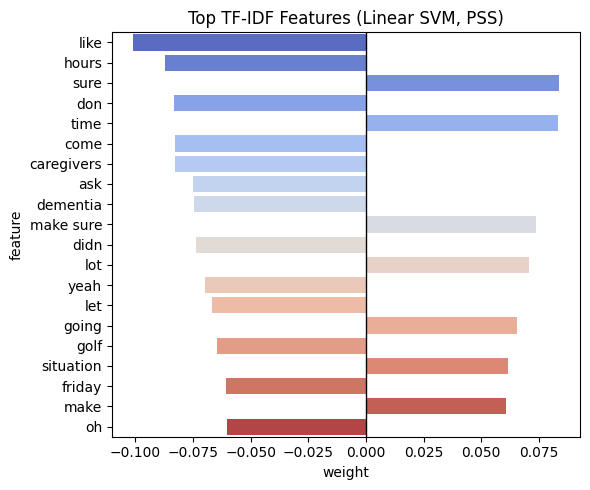
\includegraphics[width=\columnwidth]{output.png}
\caption{Top weighted TF-IDF features for PSS classification.}
\label{fig:tfidf_features}
\end{figure}

\section{Discussion}
Our study demonstrates that integrating interview data with wearable sensing provides complementary information for predicting caregiver-related outcomes. Interview data capture subjective aspects of caregivers’ psychological states, such as emotional tone and coping attitudes, while Fitbit-derived data provide objective measures of daily behavior and physiological status. Together, these sources describe complementary dimensions of caregiver well-being, and their integration improves prediction performance.

In contrast to previous studies\cite{caregiverp1,caregiverp2}, our work introduces several methodological innovations. We integrate multimodal data by combining interview-based textual information with Fitbit-derived behavioral and physiological signals, rather than relying on a single data modality. Furthermore, beyond traditional machine learning models, we explore the use of LLMs in a zero-shot setting, and design prompt engineering strategies varying along different dimensions.

Future work will include ablation studies to examine the contributions of individual modalities, including models using only wearable data or only interview data. In addition, when applying LLMs for inference, we extract the reasoning generated by the model, which may provide valuable insights into understanding and interpreting LLMs’ predictions.


\section*{Acknowledgements}
This work was supported by the National Institutes of Health (NIH) under Grant Nos. R01AG062690, K25AG070306, and R01DA059925, and by the National Science Foundation (NSF) under Grant Nos. 1840167 and 2047296. The research was conducted under the supervision of Professor Akane Sano.

\section*{CRediT Author Statement}
Junen Xiao: Methodology, Software, Formal Analysis, Data Curation, Visualization, Writing.

\section*{Code Availability}
The LaTeX source code of this report, including all files and figures required is available at:

\href{https://github.com/PepperJess99/ELEC-594/tree/main/Midterm%20Report}{GitHub repository}

\addtolength{\textheight}{-12cm}   % This command serves to balance the column lengths
                                  % on the last page of the document manually. It shortens
                                  % the textheight of the last page by a suitable amount.
                                  % This command does not take effect until the next page
                                  % so it should come on the page before the last. Make
                                  % sure that you do not shorten the textheight too much.

%%%%%%%%%%%%%%%%%%%%%%%%%%%%%%%%%%%%%%%%%%%%%%%%%%%%%%%%%%%%%%%%%%%%%%%%%%%%%%%%



%%%%%%%%%%%%%%%%%%%%%%%%%%%%%%%%%%%%%%%%%%%%%%%%%%%%%%%%%%%%%%%%%%%%%%%%%%%%%%%%

\newpage
\bibliographystyle{ieeetr}

\bibliography{reference}


\end{document}